\section{Model}
\label{sec:model}

% Sanders~\cite{sanders2009security} argues that existing security metrics should be integrated to provide a comprehensive, quantified view of systems through their lifecycle.  

 We recognize that both software quality factors, such as code size, and factors external to software development, such as the amount of money managed by the software, influence security outcomes. Software quality and external factors are multi-faceted, with multiple contributing causes. For example, software quality attributes with effects on security outcomes include code size [ref], code churn [ref], and language [ref]. External factors are not limited to the amount of money managed directly by software; attackers also focus on users and on machines.  We seek a model of the factors influencing security outcomes in software development to enable assessment of how varying security practice use affects those outcomes.

As a basis for studying how practice adherence influences security outcomes, we define structural and measurement models relating software project context, practice adherence, and security outcomes. In this section, we present the structural model constructs and how they are related, and a measurement model for how we expect observable data to link to the structural model constructs. 

\subsection{Structural Model}
  
In this section, we define conceptual constructs to model Asset Value, Software Risk, Adherence, and Outcomes, and the relationships we expect between each construct. 

\subsubsection{Asset Value}

To make claims about how security practices affect security outcomes, we need to factor out other reasons for security outcomes. While researchers have conducted studies on how various source code attributes are correlated with vulnerabilities (e.g. ),  We hypothesize that software tracking valuable or sensitive data, such as PII or credit card data is more likely to be attacked than software tracking, say, baseball scores. 

The Asset Value construct represents the characteristics of the software's purpose and usage context that may affect security Outcomes.
 

\subsubsection{Software Risk}
Software Risk represents the characteristics of the software under the control of the development team that are associated with software vulnerabilities, for example high churn and defect-prone languages. 

\subsubsection{Adherence}
\label{sec:model_contruct_adherence}
Adherence represents the efforts the team takes to prevent and discover vulnerabilities. We adapt an IEEE definition of practice~\cite{ieee1990glossary} `3. a specific type of professional or management activity that contributes to 
the execution of a process and that may employ one or more techniques and tools' to define a software development security practice to be an action a software development team member takes to prevent, identify, or resolve a vulnerability, possibly guided by a tool or reference. We measure the Adherence construct in terms of the frequency  of security practice use by the team.  
% emails - spec
% commit messages - code
% tests - test
% issues - ops
% documentation - spec

\subsubsection{Outcomes}
\label{sec:model_contruct_outcome}
The Outcomes construct represents security outcomes for the software. Meneely~\cite{meneely2016security} observes that security is negatively defined, the absence of issues in a system's confidentiality, integrity, and availability. 
However, at present, the presence of security issues, termed vulnerabilities, is the most common means of measuring security in software~\cite{morrison2014mapping}.
To describe the Outcomes construct, we begin with a definition of vulnerability. Following Krsul~\cite{krsul1998software} and Ozment~\cite{ozment2007vulnerability}, we define a software vulnerability as “an instance of a mistake in the specification, development, or configuration of software such that its execution can violate the explicit or implicit security policy.  Vulnerabilities may not only be problems in code (`bugs'~\cite{mcgraw2006software}) but may also be, for example, design issues (`flaws'), documentation issues, and configuration issues.  We distinguish between undiscovered (`latent') and discovered (`manifest') security issues.  Vulnerabilities may be manifest, when discovered by users, security researchers or the development team itself, or they may be latent, not yet discovered by users, researchers or the team. We further distinguish between vulnerabilities identified after the software is released (`Post-release'), and vulnerabilities identified before the software is released (`Pre-release'). Pre-release vulnerabilities are an indication that the development team has incorporated practices supporting discovery of vulnerabilities into its development process. Post-release vulnerabilities are an indication of both vulnerabilities that have escaped the development process and of attacker interest in the software. 

We measure the Outcomes construct in terms of manifest vulnerabilities and the timing of their discovery and resolution. Low total values for manifest vulnerabilities are preferable, and a high proportion of vulnerabilities discovered pre-release rather than post-release is also preferable. 

\subsubsection{Construct Relationships}
We hypothesize that the four constructs are related as follows:
\begin{itemize}
	\item We hypothesize that Asset Value is positively associated with negative Security Outcomes
	\item We hypothesize that Software Risk is positively associated with negative Security Outcomes
	\item We hypothesize that Practice Adherence is negatively associated with Software Risk 	
\end{itemize}

For example, a carefully-written piece of widely-used software that manages financial data (high Asset Value, low Software Risk) may have poorer Outcomes than a less well written baseball scores program used by a few hundred users (low Asset Value, high Software Risk). In an ideal world, we would expect Adherence to be correlated with Asset Value, as teams adopted security practices in proportion to the security needs of their software, its usage context, and their users. In the real word, users (especially attackers) sometimes surprise development teams in the uses of their software, unexpectedly increasing the software's Asset Value out of proportion to the team's Adherence. 

Figure~\ref{fig:model_constructs} depicts the basic construct relationships. Each circle in the figure represents a construct, modeled as a `latent variable'. We model the constructs using latent variables to indicate that our measures for each construct are aggregates of observed variables containing some level of measurement error with respect to the construct ~\cite{kline2015principles,borsboom2008latent}. Each square in the figure represents the set of observable measurements associated with each construct. We present the list of measurements for each construct in the measurement guidebook (URL on request). Each directed edge in the graph represents the influence of one construct upon another, as measured by their covariance. The weights on each edge in figure~\ref{fig:model_constructs} are from simulated data, but they represent the direction of the relationships we expect to see in empirical data, with, for example, increases in Adherence leading to reductions in Outcomes. 

\begin{figure}
		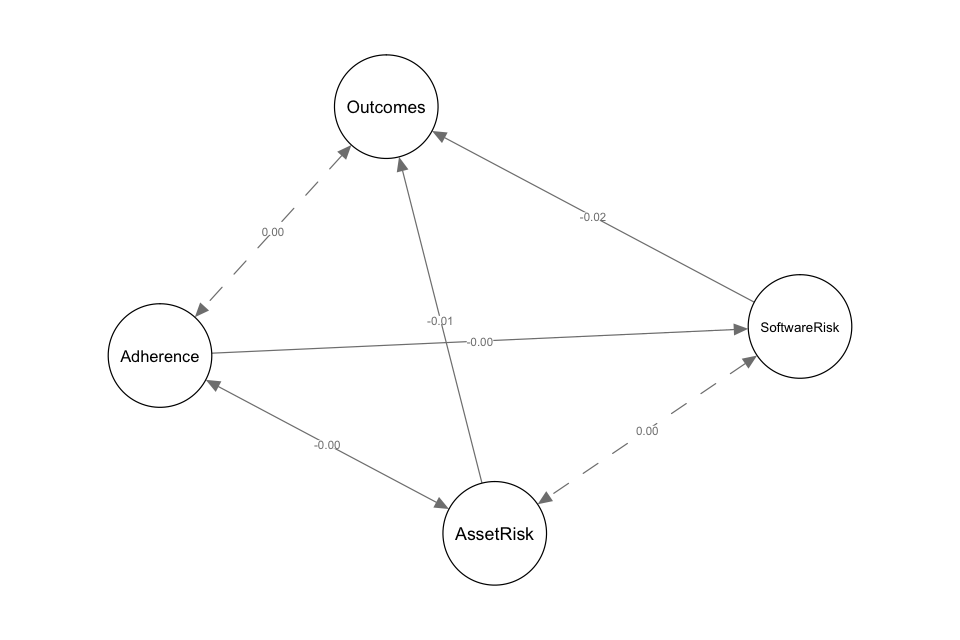
\includegraphics[width=\columnwidth]{modelzeroB}
	\caption{Structural and Measurement Model Overview}
	\label{fig:model_constructs}
\end{figure}

%\begin{figure}
% \includegraphics[width=\columnwidth]{modelcaoscto}
%	\caption{Model Constructs and Sub-Constructs}
%	\label{fig:model_constructs_phases}
%\end{figure}


\subsection{Measurement Model}
\label{sec:model_measurement}
%~\cite{morrison2014mapping}
%~\cite{morrison2016spefsite}
Through literature review and analysis, we have developed a set of measurements that we expect to capture security-related factors and outcomes for software development. To collect empirical data, we have developed a data collection framework for the measurement model, available online (URL on request). For each data element, we give our hypothesis about its relationship to the structural model construct  and name. 

\subsubsection{Software Risk}

	Language	influences	Software Risk	
	Operating System	influences	Software Risk	
	Domain	influences	Software Risk	
	Product Age	increases	Software Risk	
	SLOC	increases	Software Risk	
	Churn	increases	Software Risk	
	Team Size	influences	Software Risk	

\subsubsection{Asset Value}

	Number of Machines	increases	Asset Value
	Number of Identities	increases	Asset Value	
	Number of Dollars	increases	Asset Value	
	Source Code Availability	influences	Asset Value
	CIA Requirements	increases	Asset Value

\subsubsection{Practice Adherence}

Team Location	influences	Adherence	
Methodology	influences	Adherence	
Apply Data Classification Scheme increases	Adherence	
Apply Security Requirements		increases		Adherence
Perform Threat Modeling	increases	Adherence	
Document Technical Stack	increases	Adherence	
Apply Secure Coding Standards	increases	Adherence	
Apply Security Tooling	increases	Adherence
Perform Security Testing	increases	Adherence	
Perform Penetration Testing	increases	Adherence	
Perform Security Review	increases	Adherence	
Publish Operations Guide	increases	Adherence
Track Vulnerabilities	increases	Adherence	
Improve Development Process	increases	Adherence	
Perform Security Training	increases	Adherence	

\subsubsection{Security Outcomes}
Vulnerabilities	increase negative	Outcomes
Defects increase negative Outcomes



